% -*- TeX-master: "main"; fill-column: 72 -*-

\section{Proposed syntax and semantics}
\label{syntax}

In this section, we define the syntax and semantics of the Arrays package for SBML Level~3 Version~1.  We expound on the various data types and constructs defined in this package, then in \sect{examples}, we provide complete examples of using the constructs in example SBML models.

% -----------------------------------------------------------------------------
\subsection{Namespace URI and other declarations necessary for using this package}
\label{xml-namespace}

Every SBML Level~3 package is identified uniquely by an XML namespace URI.
For an SBML document to be able to use a given SBML Level~3 package, it
must declare the use of that package by referencing its URI.  The following
is the namespace URI for this version of the Arrays
package for SBML Level~3 Version~1:
\begin{center}
\uri{http://www.sbml.org/sbml/level3/version1/arrays/version1}
\end{center}

In addition, SBML documents using a given package must indicate whether
understanding the package is required for complete mathematical
interpretation of a model, or whether the package is optional.  This is
done using the attribute \token{required} on the \token{<sbml>} element in
the SBML document.  For the Arrays package, the value of
this attribute must be set to \val{true}.

The following fragment illustrates the beginning of a typical SBML model
using SBML Level~3 Version~1 and this version of the Arrays package:

\begin{example}
<?xml version="1.0" encoding="UTF-8"?>
<sbml xmlns="http://www.sbml.org/sbml/level3/version1/core" level="3" version="1"
      xmlns:fbc="http://www.sbml.org/sbml/level3/version1/arrays/version1" arrays:required="true">
\end{example}

\subsection{Primitive data types}
Section~3.1 of the \sbmlthreecore specification defines a number of
primitive data types and also uses a number of XML Schema 1.0 data
types~\citep{biron:2000}.  More specifically we make use of \primtype{integer}, \primtype{double}, \primtype{string}, and \primtype{SIdRef}.
% and \primtype{enum}. 
%In addition we make use of two new primitives \primtype{FbcSId} and \primtype{FbcSIdRef}, see \ref{fig:fbc_uml} for the interrelation between these entities.

% \subsubsection{Type \primtypeNC{FbcSId}}
% \label{primtype-fbcsid}

% The type \primtype{FbcSId} is derived from \primtype{SId} (\sbmlthreecore specification Section~3.1.7) and has identical syntax. The \primtype{FbcSId} type is used as the data type for the identifiers of \FluxBound (\ref{fluxbound-class}) and \Objective (\ref{objective-class}) classes. By using a separate identifier type we differentiate them from others defined in the \SBML model and thus ensuring data encapsulation. In addition the \Objective class \primtype{FbcSId} provides an identifier to the \Objective which is set as active. The equality of \primtype{FbcSId} values is determined by an exact character sequence match and therefore comparisons of these identifiers must be performed in a case-sensitive manner.

% \subsubsection{Type \primtypeNC{FbcSIdRef}}
% \label{primtype-fbcsidref}

% Type \primtype{FbcSIdRef} is used for all attributes that refer to
% identifiers of type \primtype{FbcSId}.  Derived from
% \primtype{FbcSId} it has the restriction that the value of an
% attribute having type \primtype{FbcSIdRef} must match the value of a
% \primtype{FbcSId} attribute in the current model. In the FBC package the \ListOfObjectives has an attribute of this type that is used to refer to an `active' \Objective.

\subsection{The Dimension class}

% {\bf QUESTION: SBase the right place?  If not, where can we put it so you can have an array of subModels.}
% {\bf QUESTION: lowerLImit/upperLImit, integer, SId, or math?}
%{\bf QUESTION: need a solution to the order dependence on dimensions.}

{\bf QUESTION: if we use size instead of limits, are arrays 0 based or 1 based?}

The arrays package extends several SBML L3V1 core elements with the addition of an ordered list of dimensions.  An object with a list of dimensions is an array, and the number of dimensions is equivalent to the number of array indices; a vector would have one dimension statement, a matrix two, etc.  Currently, objects are restricted to at most two dimensions.  Each dimension of an arrays has a fixed size which is with a size attribute which is a parameterId indicated with the lowerLimit and upperLimit values.  For example, a 10 by 10 array of compartments C, with array indices starting at 0, could be defined as:
\begin{verbatim} 
<parameter id="n" value="10"/>
<compartment id="C" size="1.0" ...>
 <orderedListOfDimensions>
  <dimension id="i" size="n"/>
  <dimension id="j" size="n"/>
 </orderedListOfDimensions>
</compartment>
\end{verbatim}
The scope of the dimension id is local to the enclosing object definition  (in this case the compartment) and is not visible outside the object  (compartment) definition.  
%An array lowerLimit may not exceed its upperLimit.  
% If a limit refers to a parameter with an undefined initial value than the initial value of that limit is assumed to be undefined. 
Initial values in explicit declarations for compartments, parameters, and species are assumed to refer to every element of the array.  To specify different initial values to different elements of an array an initialAssignment should be used. 

For SBML L3V1 core, the following objects are extended to include an optional ordered list of dimensions:
\begin{itemize}
\item Parameters
\item Compartments
\item Species
\item Reactions
\item Species references
\item Rules
\item Initial assignments
\item Events
\item Constraints
\end{itemize}
Packages may choose to allow dimensions as desired.  For example, comp will allow dimensions on subModels.

\begin{figure}[h]
  \centering
  % Requires \usepackage{graphicx}
  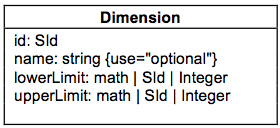
\includegraphics[width=0.5\textwidth]{images/arraysDef.png}\\
  \caption{A UML representation of the Arrays package classes. See \ref{conventions}} for conventions related to this figure. \label{fig:fbc_uml}
\end{figure}

\subsection{The Index class}

An assignment can include an ordered list of indices to specify the indices of the array element to assign to.  Currently, this list can include at most two elements of the index class.  When an element has dimensions but no index is provided, it is assumed that the entire array is referenced.  When an element has two dimensions but only one index is provided, it is assumed that the corresponding row is being referenced (TODO: need a way to get one column).  In all other cases, a scalar is returned.  Each index class object is a mathematical function that is used to compute the index.  The example below copies a reverse copy of the array in parameter x into parameter y.
\begin{verbatim} 
<parameter id="n" value="10"/>
<parameter id="x" ...>
 <orderedListOfDimensions>
  <dimension id="i" size="n"/>
 </orderedListOfDimensions>
</parameter>
<parameter id="y" ...>
 <orderedListOfDimensions>
  <dimension id="i" size="n"/>
 </orderedListOfDimensions>
</parameter>
<assignmentRule variable=y>
 <orderedListOfDimensions>
  <dimension id="i" size="m"/>
 </orderedListOfDimensions>
 <orderedListOfIndices>
  <index>
   <math>
    <apply>
     <selector/>
      <ci>y</ci>
      <apply>
       <minus/>
        <cn>11</cn>
        <ci>i</ci>
      </apply>
    </apply>
   </math>
  </index>
 </orderedListOfIndices>
 <math>
  <apply>
   <selector/>
    <ci>x</ci>
    <cn>i</cn>
  </apply>
 </math> 
</assignmentRule>
\end{verbatim}

For SBML L3V1 core, the following objects are extended to include an optional ordered list of indices:
\begin{itemize}
\item Species references
\item Rules
\item Initial assignments
\item Events assignments
\end{itemize}
Packages may choose to allow indicies as desired.  

\subsection{Extensions to the MathML subset}

In order to support arrays, the following mathML elements need to be added to the supported MathML subset. 
\begin{itemize}
\item constructors: {\bf matrix}, {\bf matrixrow}, {\bf vector}
\item element referenced operator: {\bf selector}
\item qualifier components: {\bf bvar}, {\bf lowlimit}, {\bf uplimit},  {\bf interval}, {\bf condition}
\item linear algebra operators: {\bf vectorproduct}, {\bf scalarproduct}, {\bf outerproduct}, {\bf transpose}
\item sum product operators: {\bf sum}, {\bf product}
\item quantifier operators: {\bf forall}, {\bf exists}
\end{itemize}

% {\bf QUESTION: do we need sparse arrays, conditional objects, or connection rules?}